% Native-LaTeX heatmaps generated directly from the final percentage column of
% data/oracle/oracle_category_cogrouping.csv. The CSV is ordered as a 10x10 BBQ
% matrix followed by a 19x19 MedQA matrix.
\definecolor{OracleHeatLow}{HTML}{F7FBFF}
\definecolor{OracleHeatHigh}{HTML}{125A99}
\definecolor{OracleHeatMissing}{HTML}{E3E3E3}

\ExplSyntaxOn
\ior_new:N \g_oracle_heatmap_ior
\int_new:N \l_oracle_heatmap_row_int
\int_new:N \l_oracle_heatmap_x_int
\int_new:N \l_oracle_heatmap_y_int
\tl_new:N \l_oracle_heatmap_value_tl

% #1 = first zero-based data-row index, #2 = matrix dimension.
\cs_new_protected:Npn \oracle_heatmap_draw_cells:nn #1#2
  {
    \int_zero:N \l_oracle_heatmap_row_int
    \ior_open:Nn \g_oracle_heatmap_ior
      { data/oracle/oracle_category_cogrouping.csv }
    \ior_str_map_inline:Nn \g_oracle_heatmap_ior
      {
        \int_compare:nNnT { \l_oracle_heatmap_row_int } > { 0 }
          {
            \int_set:Nn \l_tmpa_int { \l_oracle_heatmap_row_int - 1 }
            \int_compare:nT { \l_tmpa_int >= #1 }
              {
                \int_compare:nNnT { \l_tmpa_int } < { #1 + #2 * #2 }
                  {
                    \int_set:Nn \l_tmpb_int { \l_tmpa_int - #1 }
                    \int_set:Nn \l_oracle_heatmap_x_int
                      { \int_mod:nn { \l_tmpb_int } { #2 } }
                    \int_set:Nn \l_oracle_heatmap_y_int
                      { \int_div_truncate:nn { \l_tmpb_int } { #2 } }
                    \tl_set:Nn \l_oracle_heatmap_value_tl { ##1 }
                    % A greedy match removes everything through the final comma,
                    % so quoted commas in category labels do not affect parsing.
                    \regex_replace_once:nnN { \A .* , } { }
                      \l_oracle_heatmap_value_tl
                    \tl_trim_spaces:N \l_oracle_heatmap_value_tl
                    \tl_if_blank:VTF \l_oracle_heatmap_value_tl
                      {
                        \fill[OracleHeatMissing]
                          (\int_use:N\l_oracle_heatmap_x_int,
                           \int_use:N\l_oracle_heatmap_y_int)
                          rectangle ++(1,1);
                      }
                      {
                        \fill[OracleHeatHigh!
                          \tl_use:N\l_oracle_heatmap_value_tl!OracleHeatLow]
                          (\int_use:N\l_oracle_heatmap_x_int,
                           \int_use:N\l_oracle_heatmap_y_int)
                          rectangle ++(1,1);
                      }
                  }
              }
          }
        \int_incr:N \l_oracle_heatmap_row_int
      }
    \ior_close:N \g_oracle_heatmap_ior
  }
\NewDocumentCommand{\OracleHeatmapCells}{mm}
  { \oracle_heatmap_draw_cells:nn {#1}{#2} }
\ExplSyntaxOff

\newcommand{\OracleHeatmapGrid}[1]{%
  \draw[gray!25,thin] (0,0) rectangle (#1,#1);%
}

\begin{figure}[p]
  \centering
  \begin{minipage}[c]{.38\textwidth}
    \centering
    {\small\bfseries BBQ\par}
    \vspace{.35em}
    \begin{adjustbox}{max width=\linewidth}
    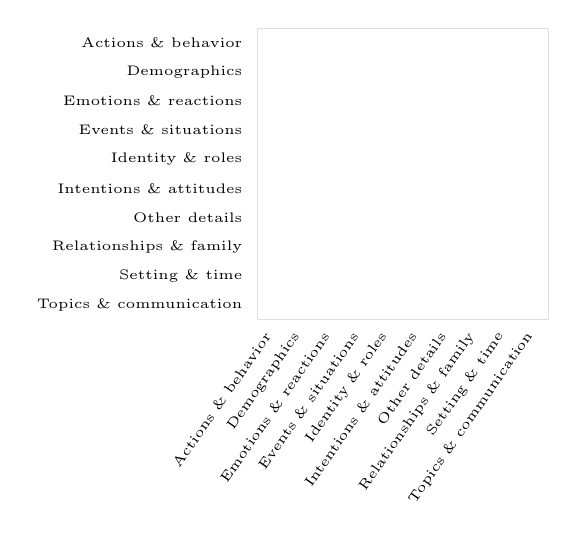
\begin{tikzpicture}[x=.37cm,y=-.37cm,
      every node/.style={font=\fontsize{5.4}{6.2}\selectfont}]
      \OracleHeatmapCells{0}{10}
      \OracleHeatmapGrid{10}
      \foreach \heatlabel [count=\i from 0] in {
        {Actions \& behavior},{Demographics},{Emotions \& reactions},
        {Events \& situations},{Identity \& roles},{Intentions \& attitudes},
        {Other details},{Relationships \& family},{Setting \& time},
        {Topics \& communication}}
        {
          \node[anchor=east] at (-.18,\i+.5) {\heatlabel};
          \node[anchor=east,rotate=55] at (\i+.55,10.22) {\heatlabel};
        }
    \end{tikzpicture}
    \end{adjustbox}
  \end{minipage}\hfill
  \begin{minipage}[c]{.60\textwidth}
    \centering
    {\small\bfseries MedQA\par}
    \vspace{.35em}
    \begin{adjustbox}{max width=\linewidth}
    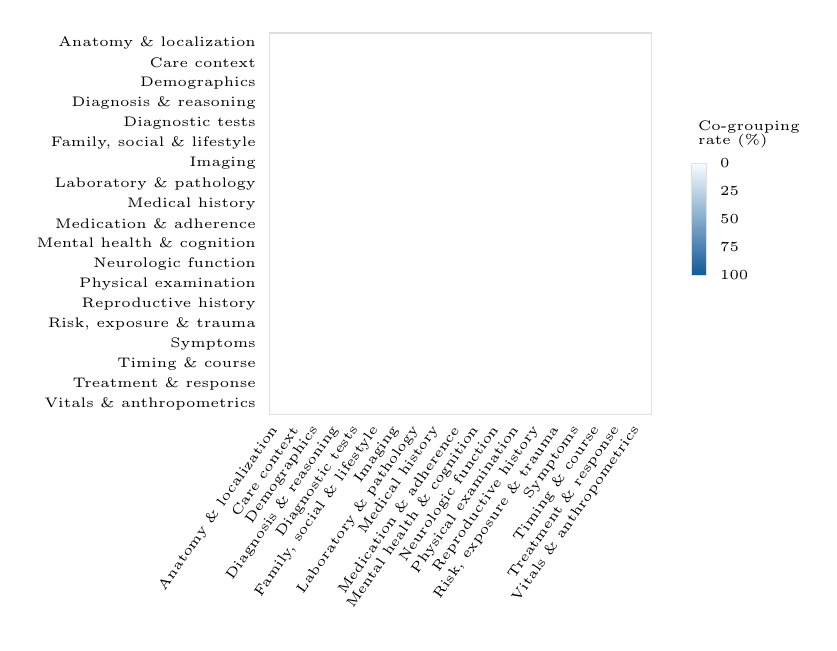
\begin{tikzpicture}[x=.255cm,y=-.255cm,
      every node/.style={font=\fontsize{4.4}{5.1}\selectfont}]
      \OracleHeatmapCells{100}{19}
      \OracleHeatmapGrid{19}
      \foreach \heatlabel [count=\i from 0] in {
        {Anatomy \& localization},{Care context},{Demographics},
        {Diagnosis \& reasoning},{Diagnostic tests},
        {Family, social \& lifestyle},{Imaging},{Laboratory \& pathology},
        {Medical history},{Medication \& adherence},
        {Mental health \& cognition},{Neurologic function},
        {Physical examination},{Reproductive history},
        {Risk, exposure \& trauma},{Symptoms},{Timing \& course},
        {Treatment \& response},{Vitals \& anthropometrics}}
        {
          \node[anchor=east] at (-.20,\i+.5) {\heatlabel};
          \node[anchor=east,rotate=55] at (\i+.55,19.25) {\heatlabel};
        }
      % Shared percentage legend.
      \foreach \p in {0,...,99}
        \fill[OracleHeatHigh!\p!OracleHeatLow]
          (21,{6.5+\p/18}) rectangle (21.75,{6.5+(\p+1)/18});
      \draw[gray!25,thin] (21,6.5) rectangle (21.75,12.0556);
      \node[anchor=south west,align=left] at (20.85,6.2)
        {Co-grouping\\rate (\%)};
      \foreach \p in {0,25,50,75,100}
        \node[anchor=west] at (21.95,{6.5+\p/18}) {\p};
    \end{tikzpicture}
    \end{adjustbox}
  \end{minipage}
  \caption{Category-level co-grouping rates for the natural-language oracle.
  Categories are LLM-normalized high-level families; color shows the conditional
  percentage of eligible within-question concept pairs assigned to the same group.
  Gray denotes that no pair from the two categories co-occurred in an evaluated
  question.}
  \label{fig:oracle-category-heatmaps}
\end{figure}
